%%%%%%%%%%%%%%%%%%%%%%%%%%%%%%%%%%%%%%%%%%%%%%%%%%%%%%%%%%%%%%%%%%%%
%%%%%%%%%%%%%%%%%%%%%%%%%%%%%%%%%%%%%%%%%%%%%%%%%%%%%%%%%%%%%%%%%%%%
%%                                                                %%
%% An example for writting your thesis using LaTeX                %%
%% Original version by Luis Costa,  changes by Perttu Puska       %%
%% Support for Swedish added 15092014                             %%
%%                                                                %%
%% This example consists of the files                             %%
%%         thesistemplate.tex (versio 2.01)                       %%
%%         opinnaytepohja.tex (versio 2.01) (for text in Finnish) %%
%%         aaltothesis.cls (versio 2.01)                          %%
%%         kuva1.eps                                              %%
%%         kuva2.eps                                              %%
%%         kuva1.pdf                                              %%
%%         kuva2.pdf                                              %%
%%                                                                %%
%%                                                                %%
%% Typeset either with                                            %%
%% latex:                                                         %%
%%             $ latex opinnaytepohja                             %%
%%             $ latex opinnaytepohja                             %%
%%                                                                %%
%%   Result is the file opinnayte.dvi, which                      %%
%%   is converted to ps format as follows:                        %%
%%                                                                %%
%%             $ dvips opinnaytepohja -o                          %%
%%                                                                %%
%%   and then to pdf as follows:                                  %%
%%                                                                %%
%%             $ ps2pdf opinnaytepohja.ps                         %%
%%                                                                %%
%% Or                                                             %%
%% pdflatex:                                                      %%
%%             $ pdflatex opinnaytepohja                          %%
%%             $ pdflatex opinnaytepohja                          %%
%%                                                                %%
%%   Result is the file opinnaytepohja.pdf                        %%
%%                                                                %%
%% Explanatory comments in this example begin with                %%
%% the characters %%, and changes that the user can make          %%
%% with the character %                                           %%
%%                                                                %%
%%%%%%%%%%%%%%%%%%%%%%%%%%%%%%%%%%%%%%%%%%%%%%%%%%%%%%%%%%%%%%%%%%%%
%%%%%%%%%%%%%%%%%%%%%%%%%%%%%%%%%%%%%%%%%%%%%%%%%%%%%%%%%%%%%%%%%%%%

%% Uncomment one of these:
%% the 1st when using pdflatex, which directly typesets your document in pdf (use jpg or pdf figures), or the 2nd when producing a ps file (use eps figures, don't use ps figures!).
\documentclass[english,12pt,a4paper,pdftex,sci,utf8]{aaltothesis}
%\documentclass[english,12pt,a4paper,dvips]{aaltothesis}

%% To the \documentclass above:
%% specify your school: arts, biz, chem, elec, eng, sci
%% specify the character encoding scheme used by your editor: utf8, latin1

%% Use one of these if you write in Finnish (see the Finnish template):
%\documentclass[finnish,12pt,a4paper,pdftex,elec,utf8]{aaltothesis}
%\documentclass[finnish,12pt,a4paper,dvips]{aaltothesis}

\usepackage{graphicx}

%% Use this if you write hard core mathematics, these are usually needed
\usepackage{amsfonts,amssymb,amsbsy,csquotes}

% \usepackage[backend=biber,natbib=true,style=numeric-comp,sorting=none]{biblatex}
\usepackage{biblatex}
\addbibresource{./refs.bib}

%% Use the macros in this package to change how the hyperref package below typesets its hypertext -- hyperlink colour, font, etc. See the package documentation. It also defines the \url macro, so use the package when not using the hyperref package.
%\usepackage{url}

%% Use this if you want to get links and nice output. Works well with pdflatex.
\usepackage{hyperref}
\hypersetup{pdfpagemode=UseNone, pdfstartview=FitH,
  colorlinks=true,urlcolor=red,linkcolor=blue,citecolor=black,
  pdftitle={Default Title, Modify},pdfauthor={Your Name},
  pdfkeywords={Modify keywords}}


%% All that is printed on paper starts here
\begin{document}

%% Change the school field to specify your school if the automatically set name is wrong
% \university{aalto-yliopisto}
% \university{aalto University}
% \school{Sähkötekniikan korkeakoulu}
% \school{School of Electrical Engineering}

%% Only for B.Sc. thesis: Choose your degree programme.
%\degreeprogram{Electronics and electrical engineering}

%% ONLY FOR M.Sc. AND LICENTIATE THESIS: Specify your department,
%% professorship and professorship code.
\department{Department of Computer Science}
\professorship{Computer Science}
%%

%% Valitse yksi näistä kolmesta
%%
%% Choose one of these:
%\univdegree{BSc}
\univdegree{MSc}
%\univdegree{Lic}

%% Your own name (should be self explanatory...)
\author{Aarni Halinen}

%% Your thesis title comes here and again before a possible abstract in
%% Finnish or Swedish . If the title is very long and latex does an
%% unsatisfactory job of breaking the lines, you will have to force a
%% linebreak with the \\ control character.
%% Do not hyphenate titles.
%%
\thesistitle{Kubernetes inter-pod container isolation}

\place{Espoo}

%% For B.Sc. thesis use the date when you present your thesis.
\date{1.6.2023}

%% B.Sc. or M.Sc. thesis supervisor
%% Note the "\" after the comma. This forces the following space to be a normal interword space, not the space that starts a new sentence.
%% This is done because the fullstop isn't the end of the sentence that should be followed by a slightly longer space but is to be followed by a regular space.
\supervisor{Prof.\ Mario Di Francesco} %{Prof.\ Pirjo Professori}

%% B.Sc. or M.Sc. thesis advisors(s). You can give upto two advisors in this template. Check with your supervisor how many official advisors you can have.
\advisor{M.Sc.\ (Tech.)\ José\ Luis\ Martin\ Navarro}
\advisor{M.Sc.\ (Tech.)\ Jacopo\ Bufalino}

%% Aalto logo: syntax:
%% \uselogo{aaltoRed|aaltoBlue|aaltoYellow|aaltoGray|aaltoGrayScale}{?|!|''}
%%
%% Logo language is set to be the same as the document language.
%% Logon kieli on sama kuin dokumentin kieli
\uselogo{aaltoRed}{''}

%% Create the coverpage
\makecoverpage

%% Note that when writting your master's thesis in English, place
%% the English abstract first followed by the possible Finnish abstract

%% English abstract.
%% All the information required in the abstract (your name, thesis title, etc.)
%% is used as specified above.
%% Specify keywords
\keywords{Kubernetes, Container, Docker, Security}
%% Abstract text
\begin{abstractpage}[english]
  Your abstract in English. Try to keep the abstract short; approximately
  100 words should be enough. The abstract explains your research topic,
  the methods you have used, and the results you obtained.
  Your abstract in English. Try to keep the abstract short; approximately
  100 words should be enough. The abstract explains your research topic,
  the methods you have used, and the results you obtained.

  Your abstract in English. Try to keep the abstract short; approximately
  100 words should be enough. The abstract explains your research topic,
  the methods you have used, and the results you obtained.
  Your abstract in English. Try to keep the abstract short; approximately
  100 words should be enough. The abstract explains your research topic,
  the methods you have used, and the results you obtained.
\end{abstractpage}

%% Force a new page so that the possible English abstract starts on a new page
\newpage
%
%% Abstract in Finnish.  Delete if you don't need it.
% \thesistitle{Opinnäyteohje}
% \advisor{TkT Olli Ohjaaja}
% \degreeprogram{Electronics and electrical engineering}
% \department{Radiotieteen ja -tekniikan laitos}
% \professorship{Piiriteoria}
% %% Avainsanat
% \keywords{Vastus, Resistanssi,\\ Lämpötila}
% %% Tiivistelmän tekstiosa
% \begin{abstractpage}[finnish]
%   Tiivistelmässä on lyhyt selvitys (noin 100 sanaa)
%   kirjoituksen tärkeimmästä sisällöstä: mitä ja miten on tutkittu,
%   sekä mitä tuloksia on saatu.
%   Tiivistelmässä on lyhyt selvitys (noin 100 sanaa)
%   kirjoituksen tärkeimmästä sisällöstä: mitä ja miten on tutkittu,
%   sekä mitä tuloksia on saatu.

%   Tiivistelmässä on lyhyt selvitys (noin 100 sanaa)
%   kirjoituksen tärkeimmästä sisällöstä: mitä ja miten on tutkittu,
%   sekä mitä tuloksia on saatu.
%   Tiivistelmässä on lyhyt selvitys (noin 100 sanaa)
%   kirjoituksen tärkeimmästä sisällöstä: mitä ja miten on tutkittu,
%   sekä mitä tuloksia on saatu.
%   Tiivistelmässä on lyhyt selvitys (noin 100 sanaa)
%   kirjoituksen tärkeimmästä sisällöstä: mitä ja miten on tutkittu,
%   sekä mitä tuloksia on saatu.
% \end{abstractpage}

% \newpage

\mysection{Preface}
I want to thank Professor Pirjo Professori
and my instructor Olli Ohjaaja for their
good and poor guidance.\\

\vspace{5cm}
Otaniemi, 16.1.2015

\vspace{5mm}
{\hfill Eddie E.\ A.\ Engineer \hspace{1cm}}

%% Force new page after preface
\newpage

%% Table of contents.
\thesistableofcontents

%% Symbols and abbreviations
\mysection{Symbols and abbreviations}

\subsection*{Symbols}

\begin{tabular}{ll}
$\uparrow$       & electron spin direction up\\
$\downarrow$     & electron spin direction down
\end{tabular}

\subsection*{Operators}

\begin{tabular}{ll}
$\nabla \times \mathbf{A}$              & curl of vectorin $\mathbf{A}$\\
\end{tabular}

\subsection*{Abbreviations}

\begin{tabular}{ll}
K8s         & Kubernetes \\
STRIDE      & an object-oriented analog circuit simulator and design tool \\
\end{tabular}


%% Tweaks the page numbering to meet the requirement of the thesis format:
%% Begin the pagenumbering in Arabian numerals (and leave the first page
%% of the text body empty, see \thispagestyle{empty} below).
%% Additionally, force the actual text to begin on a new page with the
%% \clearpage command.
%% \clearpage is similar to \newpage, but it also flushes the floats (figures
%% and tables).
%% There is no need to change these
\cleardoublepage
\storeinipagenumber
\pagenumbering{arabic}
\setcounter{page}{1}

\section{Introduction}

%% Leave first page empty
\thispagestyle{empty}

T\"am\"an tekstin l\"ahteen\"a oleva tiedosto on opinn\"aytteen
pohja, jota voi k\"aytt\"a\"a kandidaatinty\"oss\"a, diplomity\"oss\"a ja
lisensiaatinty\"oss\"a. Tekstin
l\"ahteen\"a oleva tiedosto on kirjoitettu  \LaTeX-tiedoston rakenteen
opiskelemista ajatellen. Tiedoston kommentit sis\"alt\"av\"at
tietoa, joka on hy\"odyllist\"a opinn\"aytett\"a kirjoitettaessa.

%% Esimerkki luettelosta. Lyhyt ajatusviiva on k\"ayt\"oss\"a
%% luettelossa, ja se on pituudeltaan
%% en dash. Merkit\"a\"an latex-koodissa --.
Johdanto selvitt\"a\"a samat asiat kuin tiivistelm\"a, mutta
laveammin. Johdannossa kerrotaan yleens\"a seuraavat asiat

\begin{itemize}
\item[--]Tutkimuksen taustaa ja tutkimusaiheen yleisluonteinen esittely
\item[--]Tutkimuksen tavoitteet
\item[--]P\"a\"akysymys ja osaongelmat
\item[--]Tutkimuksen rajaus ja keskeiset k\"asitteet.
\end{itemize}

Lyhyiden opinn\"aytteiden johdannot ovat yleens\"a liian pitki\"a, joten
johdannon paisuttamista on v\"altett\"av\"a. Diplomity\"oh\"on sopii johdanto,
joka on 2--4 sivua. %% t\"ass\"a on my\"os lyhyt ajatusviiva l. en dash.
Kandidaatinty\"on johdannon on oltava diplomity\"on
johdantoa lyhyempi. Sopivasti tiivistetty johdanto ei kaipaa alaotsikoita.


%% In a thesis, every section starts a new page, hence \clearpage
\clearpage

\section{Background}

\subsection{Principle of least priviledge, Zero trust...}

\subsection{Microservices architecture}
\subsection{Containerization and Docker}

\begin{figure}[h!]
  \centering
  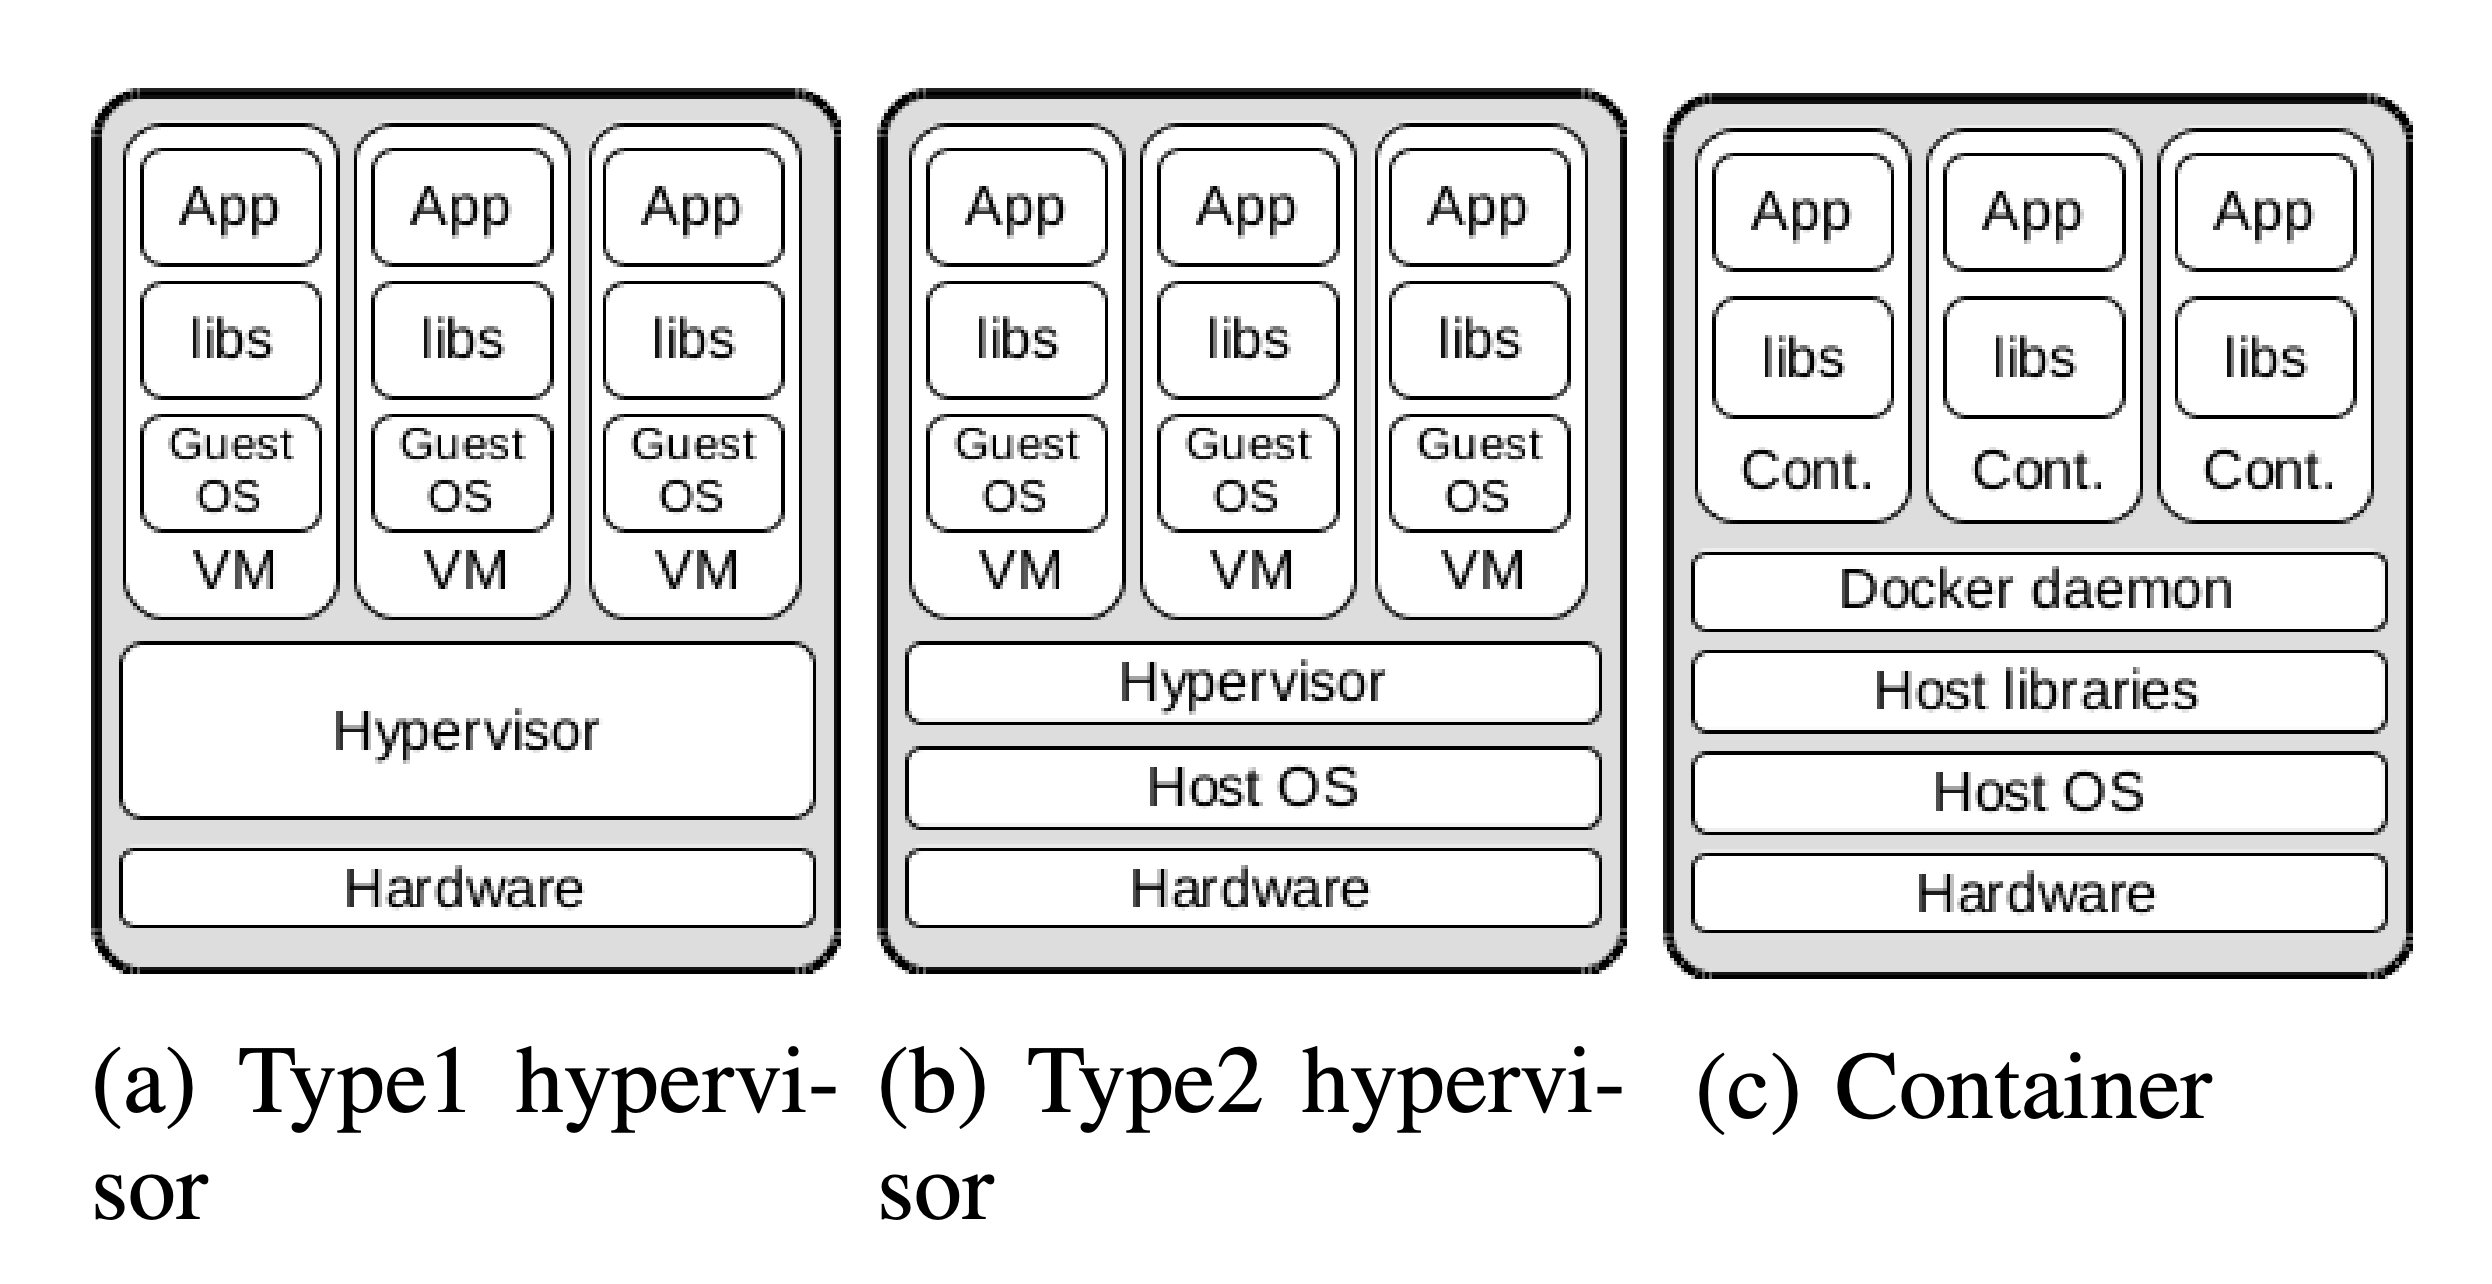
\includegraphics[width=\linewidth]{files/figure-1.png}
  \caption{Virtualization models \cite{combe2016docker}}
  \label{figure-1}
\end{figure}

Different virtualization models are illustrated in figure~\ref{figure-1}. Whereas traditional virtualization techniques virtualize workloads on top of a hypervisor which shares hardware resources between the virtual machines, containerization is a technique where virtualization happens on a operating system level \cite{merkel2014docker}. Processes executing in containers run on the host machine kernel. However, each container is isolated to its own network, process namespace and so on; two containers on the same host OS do not know that they share resources. Furthermore, containers are similarly isolated from accessing host OS resources.

BSD jails and \textit{chroot} can be considered early forms of containerization technology, so the idea of containers is not new \cite{combe2016docker}. Recent Linux container solutions rely on two main implementations: Linux Containers (LXC) -based solution that relies on kernel features such as control groups (cgroups) and namespaces, and a custom kernel and Linux distribution called Open Virtuozzo (OpenVZ). Docker \cite{docker} is a hugely popular container runtime that is based on LXC and provides an easy-to-use API and tooling for creating and managing containers. Docker also provides containerization for other OSes as well. However, in this thesis we focus only on the Linux implementation.

\subsubsection{Linux containers}
6 ns:
mnt
pid
net
ipc
uts (hostname)
user (UIDs)

control groups for resource management

\subsubsection{Linux capabilities, priviledged containers, Container breakout}
\subsubsection{Docker}

\cite{bui2015analysis}

\begin{enumerate}
  \item Priviledged container
  \item CAP\_SYS\_ADMIN, mounting /proc and chroot
  \item CAP\_SYS\_PTRACE, shellcode injection to running program, nc 172.17.0.1 on port running shell
  \item Mounted docker socket, creating priviledged containers
\end{enumerate}


\subsection{Kubernetes system components, control plane}
\subsubsection{apiserver}
\subsubsection{etcd}
\subsubsection{scheduler}
\subsubsection{controller-manager}

\subsection{Kubernetes resources}
\subsubsection{Namespaces}
\subsubsection{Pods}
\subsubsection{Services}
\subsubsection{Admission control}

\subsection{Kubernetes network model}

% https://kubernetes.io/docs/concepts/services-networking/
% https://kubernetes.io/docs/concepts/extend-kubernetes/compute-storage-net/network-plugins/

% The key requirements of the Kubernetes network model include i) Pods are IP addressable and must be able to communicate with all other Pods (on the same or different host) without the need for network address translation (NAT), and ii) all the agents on a host (e.g., Kubelet) are able to communicate with all the Pods on that host. CNI plugins may differ in their architecture but meet the above network rules.

Integral part of Kubernetes cluster is how nodes and resources are networked together. Specifically, the networking model needs to address four different type of networking problems: i) intra-Pod (ie. container-to-container within same Pod) communication, ii) inter-Pod communication between Pods, iii) Service-to-Pod communication and iv) communication from external sources to Services \cite{k8s-docs-cluster-networking}. The model also requires that each Pod is IP addressable and can communicate with other Pods without network address translation (NAT), even when Pods are scheduled on different hosts \cite{qi2020assessing}. All agents on a host should also be able to communicate with Pods on the same host. The implementation of this model is not part of Kubernetes, but is handed to special plugins that implement Container Network Interface (CNI) specification.

% When a new Pod is added, the CNI plugin coordinates with the container runtime and connects the container network namespace with the host network namespace (e.g., , veth pair), assigns a unique IP address to the new Pod, applies the desired network policies and distributes routing information to the rest of the cluster.

% https://www.tkng.io/cni/

% Connectivity - making sure that a Pod gets its default eth0 interface with IP reachable from the root network namespace of the hosting Node.
% Reachability - making sure that Pods from other Nodes can reach each other directly (without NAT).

% Connectivity requirement is the most straight-forward one to understand – every Pod must have a NIC to communicate with anything outside of its own network namespace. Some local processes on the Node (e.g. kubelet) need to reach PodIP from the root network namespace (e.g. to perform health and readiness checks), hence the root NS connectivity requirement.

% Reachability, on the other hand, may require a bit of unpacking:
% - Every Pod gets a unique IP from a PodCIDR range configured on the Node.
% - This range is assigned to the Node during kubelet bootstrapping phase.
% - Nodes are not aware of PodCIDRs assigned to other Nodes, allocations are normally managed by the controller-manager based on the --cluster-cidr configuration flag.
% - Depending on the type of underlying connectivity, establishing end-to-end reachability between PodCIDRs may require different methods:
%   - If all Nodes are in the same Layer2 domain, the connectivity can be established by configuring a full mesh of static routes on all Nodes with NextHop set to the internal IP of the peer Nodes.
%   - If some Nodes are in different Layer2 domains, the connectivity can be established with either:
%     - Orchestrating the underlay – usually done with BGP for on-prem or some form of dynamically-provisioned static routes for public cloud environments.
%     - Encapsulating in the overlay – VXLAN is still the most popular encap type.

\subsubsection{Container Network Interface}

The Container Network Interface (CNI) \cite{cni} is a networking specification, which has become de facto industry standard for container networking. It is backed by Cloud Nativce Computing Foundation (CNCF) \cite{qi2020assessing}. CNI was first developed for the container runtime \texttt{rkt}, but it is supported by all container runtimes and there is a large number of implementations to choose from \cite{hausenblas2018container}. Most of the container orchestrators have adopted the specification as their networking solution. The biggest outlier is Docker Swarm, which instead implements \texttt{libnetwork} \cite{libnetwork}.

The specification has five distinct definitions: i) a format for network configuration, ii) a execution protocol between the container runtimes and the plugin binary, iii) a procedure for the runtime to interpret the configuration and execute the plugins, iv) a procedure for deletegating functionality between the plugins and v) data types for plugins to return their results to the runtime \cite{cni}. The configuration is defined as a JSON file and it includes a list of plugins and their configuration. The file is consumed at plugin execution time by the runtime, and passed to the plugins. The execution protocol defines a set of operations (ADD, DEL, CHECK) for adding and removing containers from the network, while also defining a set of OS environment variables that are used as parameters by the plugins. When the runtime mutates a container network, it results in a series of ADD, DELETE or CHECK executions. These are then executed in same order as defined in the \texttt{plugins} list, or reversed order for DELETE executions. Each plugin then returns either \texttt{Success} or \texttt{Error} JSON object. The execution of a series of operations ends when it encounters the first Error response, or when all the operations have been performed.

% Kubernetes Network Policy is the means to enforce rules
% indicating which network traffic is allowed and which Pods
% can communicate with each other. The policies applied to Pod
% network traffic can be based on their applicability to ingress
% traffic (entering the Pod) and egress traffic (outgoing traffic).
% The control strategies include “allow” and “deny”. By default,
% a Pod is in a non-isolated state. Once a network policy is
% applied to a Pod, all traffic that is not explicitly allowed will
% be rejected by the network policy. However, other Pods that do
% not have network policies applied to them are not affected. CNI
% plugins in Kubernetes can implement elaborate traffic control
% and isolation mechanisms.

% Network policies help to provide the guardrails needed to
% restrict traffic between pods (in and/or across namepaces) as
% well as between pods and external networks, by explicitly
% specifying allowed and denied connections. A network policy
% specification consists of a podSelector to specify pods
% that will be subject to the policy and policyTypes to
% specify the types of policies, i.e., ingress and/or egress. Ingress
% rules specify allowed inbound traffic to the target pods, and
% egress rules specify allowed outbound traffic from the target
% pods. Each rule is comprised of a NetworkPolicyPeer
% for selecting pods on the other side of the connection to/from
% which traffic is allowed, through a Classless Inter-Domain
% Routing (CIDR) notation that specifies IP address blocks,
% namespaces, or pod labels; and a NetworkPolicyPort
% that allows to explicitly specify ports or protocols that may
% communicate with the pod. Network policies are additive, and
% if multiple policies select a pod, traffic is restricted to what is
% allowed by the union of those policies’ ingress/egress rules.

\subsubsection{Network policies}

Since Kubernetes does not provide networking between the Pods, it has no capabilities to enforce network isolation between workloads. Thus, another key feature for CNI plugins is enforcing network traffic rules. Kubernetes provides a common resource called \texttt{NetworkPolicy} for CNI plugins to consume. The NetworkPolicy specification consists of a \texttt{podSelector} that specifies pods that are subject to the policy and \texttt{policyTypes} to specify Ingress and Egress rules for the traffic \cite{budigiri2021network} to the target Pod. Each rule includes \texttt{to} or \texttt{from} field for selecting Pod, Namespace or IP address block in CIDR notation on the other side of the connection, and \texttt{ports} field for explicitly specifying which ports and protocols are part of the rule. The policies are additive; when multiple rules are defined for a Pod, the traffic is restricted to what is allowed by the union of the policies. Many CNI plugins also introduce Custom Resource Definitions for their own, more granular, network policy rules.

\subsubsection{Cilium and other CNI plugins}

TODO: CNI plugins, daemons and binary \cite{qi2020understanding}.

While all CNI plugins meet the requirements listed above, they may differ in architecture significantly. The plugins can be classified based on which OSI model network layer they operate on, which Linux kernel features they use for packet filtering and which encapsulation and routing model they support for inter-host and intra-host communication between Pods.

In this thesis, we focus on three different CNI plugins: Cilium, Calico and Multus.

Cilium \cite{cilium} is one of the most advanced and powerful CNI plugins for Kubernetes. It works by creating virtual ethernet device for each Pod and sets one side of the link into Pod's network namespace \cite{cilium-tkng}. Cilium then attaches extended Berkeley Packet Filter (eBPF) programs to ingress traffic control (\texttt{tc}) hooks of these virutal ethernet devices for intercepting all incoming packets from the Pod. The packets are intercepted and processed before the network stack and thus \texttt{iptables}, reducing latency 20\%-30\% and even doubling the throughput of packets in some scenarios \cite{budigiri2021network}.

Cilium provides Custom Resource Definition \texttt{CiliumNetworkPolicy} that supports policies in layers 3-7 instead of standard L3/L4. With \texttt{CiliumClusterwideNetworkPolicy}, network rules can applied to every namespace in the cluster, or even to nodes when using \texttt{nodeSelector}.

\subsubsection{Extended Berkeley Packet Filter}

Berkeley Packet Filter (BPF, or nowadays often cBPF) was originally developed in early 1990s as a high-performance tool for user-space packet captures \cite{mccanne1993bsd}. BPF works by deploying the filtering part of the application, \texttt{packet filter}, in the kernel-space as an agent. The \texttt{packet filter} is provided with a program (often denoted as BPF program) consisting of BPF instructions, which works as a set of rules for selecting which packets are of interest in the user-space application and should be copied from kernel-space to user-space. The instuctions are executed in a register-based pseudo machine. Since network monitors are often interested only in subset of network traffic, this limits the number of expensive copy operations across the kernel/user-space protection boundary only to packets that are of interest in the user-space application. A notable usecase for BPF is \textit{libpcap} library, which is used by network monitoring tool called \texttt{tcpdump}.

Later in the 2010s the Linux community realized that BPF and it's ability to instrument the kernel could benefit other areas than packet filtering as well \cite{vieira2020fast}. This reworked version of BPF was first merged in to Linux kernel in 2014 and is publicly called extended Berkeley Packet Filter (eBPF) to distinguish it from the original cBPF. The kernel development community continues to call the newer version BPF, but instead of the original acronym consider it a name of a technology. Similarly to the kernel community, the term BPF always refers to the eBPF in this thesis.

The eBPF programs are compiled to bytecode and loaded to kernel with \texttt{bpf()} system call \cite{miano2021framework}. Most often programs are written in restricted C and compiled with LLVM Clang compiler to bytecode. It also possible to use eBPF assembly instructions and \texttt{bpf\_asm} utility for converting instructions to bytecode. eBPF programs follow a event-driven architecture: a loaded eBPF program is hooked to a particular type of event and each occurence of the event triggers the program execution.

% TODO: Yhidstä johonkin kappaleeseen
For networking purposes, there are two eBPF hooks available for intercepting and mangling, forwarding or dropping network packets: eXpress Data Path (XDP) and Traffic Control (TC) \cite{miano2021framework}. In Cloudflares DDoS testing benchmark \cite{cloudflare-xdp}, XDP program was capable to drop 10 million and TC program 2 million packets per second, while common \texttt{iptables} INPUT rule was able to drop less than one million packets per second.

XDP programs are attached to a network interface controller (NIC) and can handle only incoming packets \cite{hoiland2018express}. The programs are called directly by the NIC driver if it has XDP support, thus executing before packets enters the network stack. This skips expensive packet parsing and memory allocation operations, and allow XDP programs to run at very high throughput. Thus, even the main networking buffer \textit{skbuff} is not populated. Some SmartNICs even support offloading the program to the NIC's own processor from host CPU, improving host machine performance even further \cite{cilium-program-types}. If the driver does not support XDP, generic XDP is used and the programs run after the packet has been parsed by the network stack.

XDP programs can read and modify contents of the packets \cite{vieira2020fast}. Since the packets are not parsed the network stack, the programs have to work with raw packets and implement own parsing functionality. The program's return value determines how the packet should be processed further. With \texttt{XDP\_DROP} and \texttt{XDP\_PASS} return values, the packet can be dropped or passed further to the networking stack respectively. The packet can also be bounced back to the same NIC it arrived on with \texttt{XDP\_TX}, usually after modifying the packet contents. \texttt{XDP\_REDIRECT} is used for redirecting the packet to a different NIC, CPU or even to another socket.

TC programs are executed when both incoming and outgoing packets reach kernel traffic control function within the Linux network stack \cite{vieira2020fast}. The ingress hook executes after the packet is parsed to \textit{skbuff} but before most of the network stack. On egress the stack is traversed in reverse, thus the hook executes after most of the network stack. TC programs can read and write directly to packet in memory. Similarly to XDP programs, the return value of the program determines further processing of the packet. The packet can be passed furhter in the stack with \texttt{TC\_ACT\_OK}, dropped with \texttt{TC\_ACT\_SHOT}, or the modified packet can be redirected back to the start of the classification with \texttt{TC\_ACT\_RECLASSIFY}, among others.

\clearpage

\section{Research material and methods}

T\"ass\"a osassa kuvataan k\"aytetty tutkimusaineisto ja
tutkimuksen metodologiset valinnat, sek\"a
kerrotaan tutkimuksen toteutustapa ja k\"aytetyt menetelm\"at.

\clearpage

\section{Evaluation}

T\"ass\"a osassa esitet\"a\"an tulokset ja vastataan tutkielman alussa
esitettyihin tutkimuskysymyksiin. Tieteellisen kirjoitelman
arvo mitataan t\"ass\"a osassa esitettyjen tulosten perusteella.

Tutkimustuloksien merkityst\"a on aina syyt\"a arvioida ja tarkastella
kriittisesti.  Joskus tarkastelu voi olla t\"ass\"a osassa, mutta se
voidaan my\"os j\"att\"a\"a viimeiseen osaan, jolloin viimeisen osan nimeksi
tulee >>Tarkastelu>>. Tutkimustulosten merkityst\"a voi arvioida my\"os
>>Johtop\"a\"at\"okset>>-otsikon alla viimeisess\"a osassa.

T\"ass\"a osassa on syyt\"a my\"os arvioida tutkimustulosten luotettavuutta.
Jos tutkimustulosten merkityst\"a arvioidaan >>Tarkastelu>>-osassa,
voi luotettavuuden arviointi olla my\"os siell\"a.

\clearpage

\section{Conclusion}

Opinn\"aytteen tekij\"a vastaa siit\"a, ett\"a opinn\"ayte on t\"ass\"a dokumentissa
ja opinn\"aytteen tekemist\"a k\"asittelevill\"a luennoilla sek\"a
harjoituksissa annettujen ohjeiden mukainen muotoseikoiltaan,
rakenteeltaan ja ulkoasultaan.

\clearpage

%% The \phantomsection command is nessesary for hyperref to jump to the correct page, in other words it puts a hyper marker on the page.
\phantomsection

\thesisbibliography
\printbibliography

%% Appendices
\clearpage

\thesisappendix

\section{Esimerkki liitteest\"a\label{LiiteA}}

Liitteet eiv\"at ole opinn\"aytteen kannalta v\"altt\"am\"att\"omi\"a ja
opinn\"aytteen tekij\"an on
kirjoittamaan ryhtyess\"a\"an hyv\"a ajatella p\"arj\"a\"av\"ans\"a ilman liitteit\"a.
Kokemattomat kirjoittajat, jotka ovat huolissaan
tekstiosan pituudesta, paisuttavat turhan
helposti liitteit\"a pit\"a\"akseen tekstiosan pituuden annetuissa rajoissa.
T\"all\"a tavalla ei synny hyv\"a\"a opinn\"aytett\"a.

\clearpage

\end{document}